\documentclass[../main.tex]{subfiles}

\begin{document}
\subsection{Gondola Arm Stresses} \label{bearingArm}
The failure of the gondola arm will be analysed as shown in Figure \ref{fig:deflection}. 

\begin{figure}[H]
	\centering
	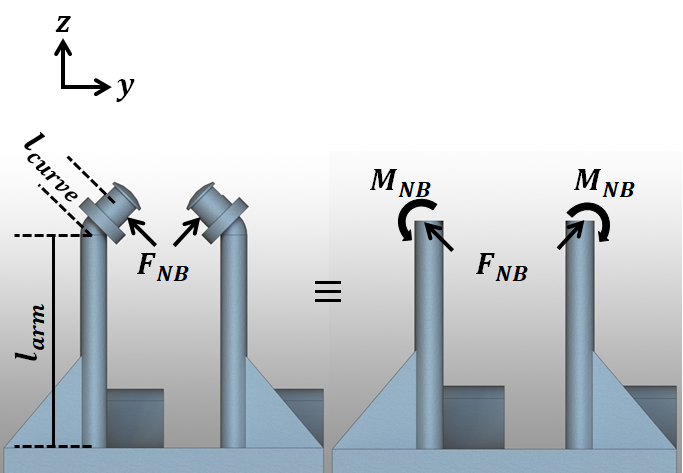
\includegraphics[width=.8\linewidth]{img/gondola/armDeflection.PNG}
	\caption{Model Used to Compute the Deflection of the Gondola Arms}
	\label{fig:deflection}
\end{figure}

For the sake of simplicity, the curved section at the very top is ignored and the force is translated from the curved section to the straight section using a force-moment couple. The moment $M_{NB}$ is computed as $M_{NB}=F_{NB}l_{curve}$. Furthermore, the rib seen in Figure \ref{fig:deflection} is ignored. The failure criteria will be computed without the rib, and the rib will be added as an extra preventative measure, to ensure the member is rigid enough.\\

\begin{align}
	\sigma _{Gondola Arm} = \sigma _{axial} + \sigma _{bending force} + \sigma _{bending moment} \\ \label{armStress}
	\sigma _{Gondola Arm}  = \left(\dfrac{F_{NB_{z}}}{A}\right)\hat{k} + \left(\dfrac{F_{NB_{y}}l_{arm}c}{I}  + \dfrac{M_{NB}c}{I} \right) \hat{j}
\end{align}

These stresses are converted to principle stresses (as shown in Appendix \ref{appendix:cauchy}). These principle stresses are then used to determine the safety factor by Brittle Mohr-Coulomb Theory \cite[227]{shigley}.

Since $\sigma _a > \sigma _b > 0$,

\begin{equation}
	\eta = \dfrac{S_{ut}}{\sigma _a} \Rightarrow 1.5 \geq \dfrac{S_{ut}}{\sigma _a}
\end{equation}

\end{document}